\begin{figure*}
\centering

\begin{subfigure}{\textwidth}
\centering
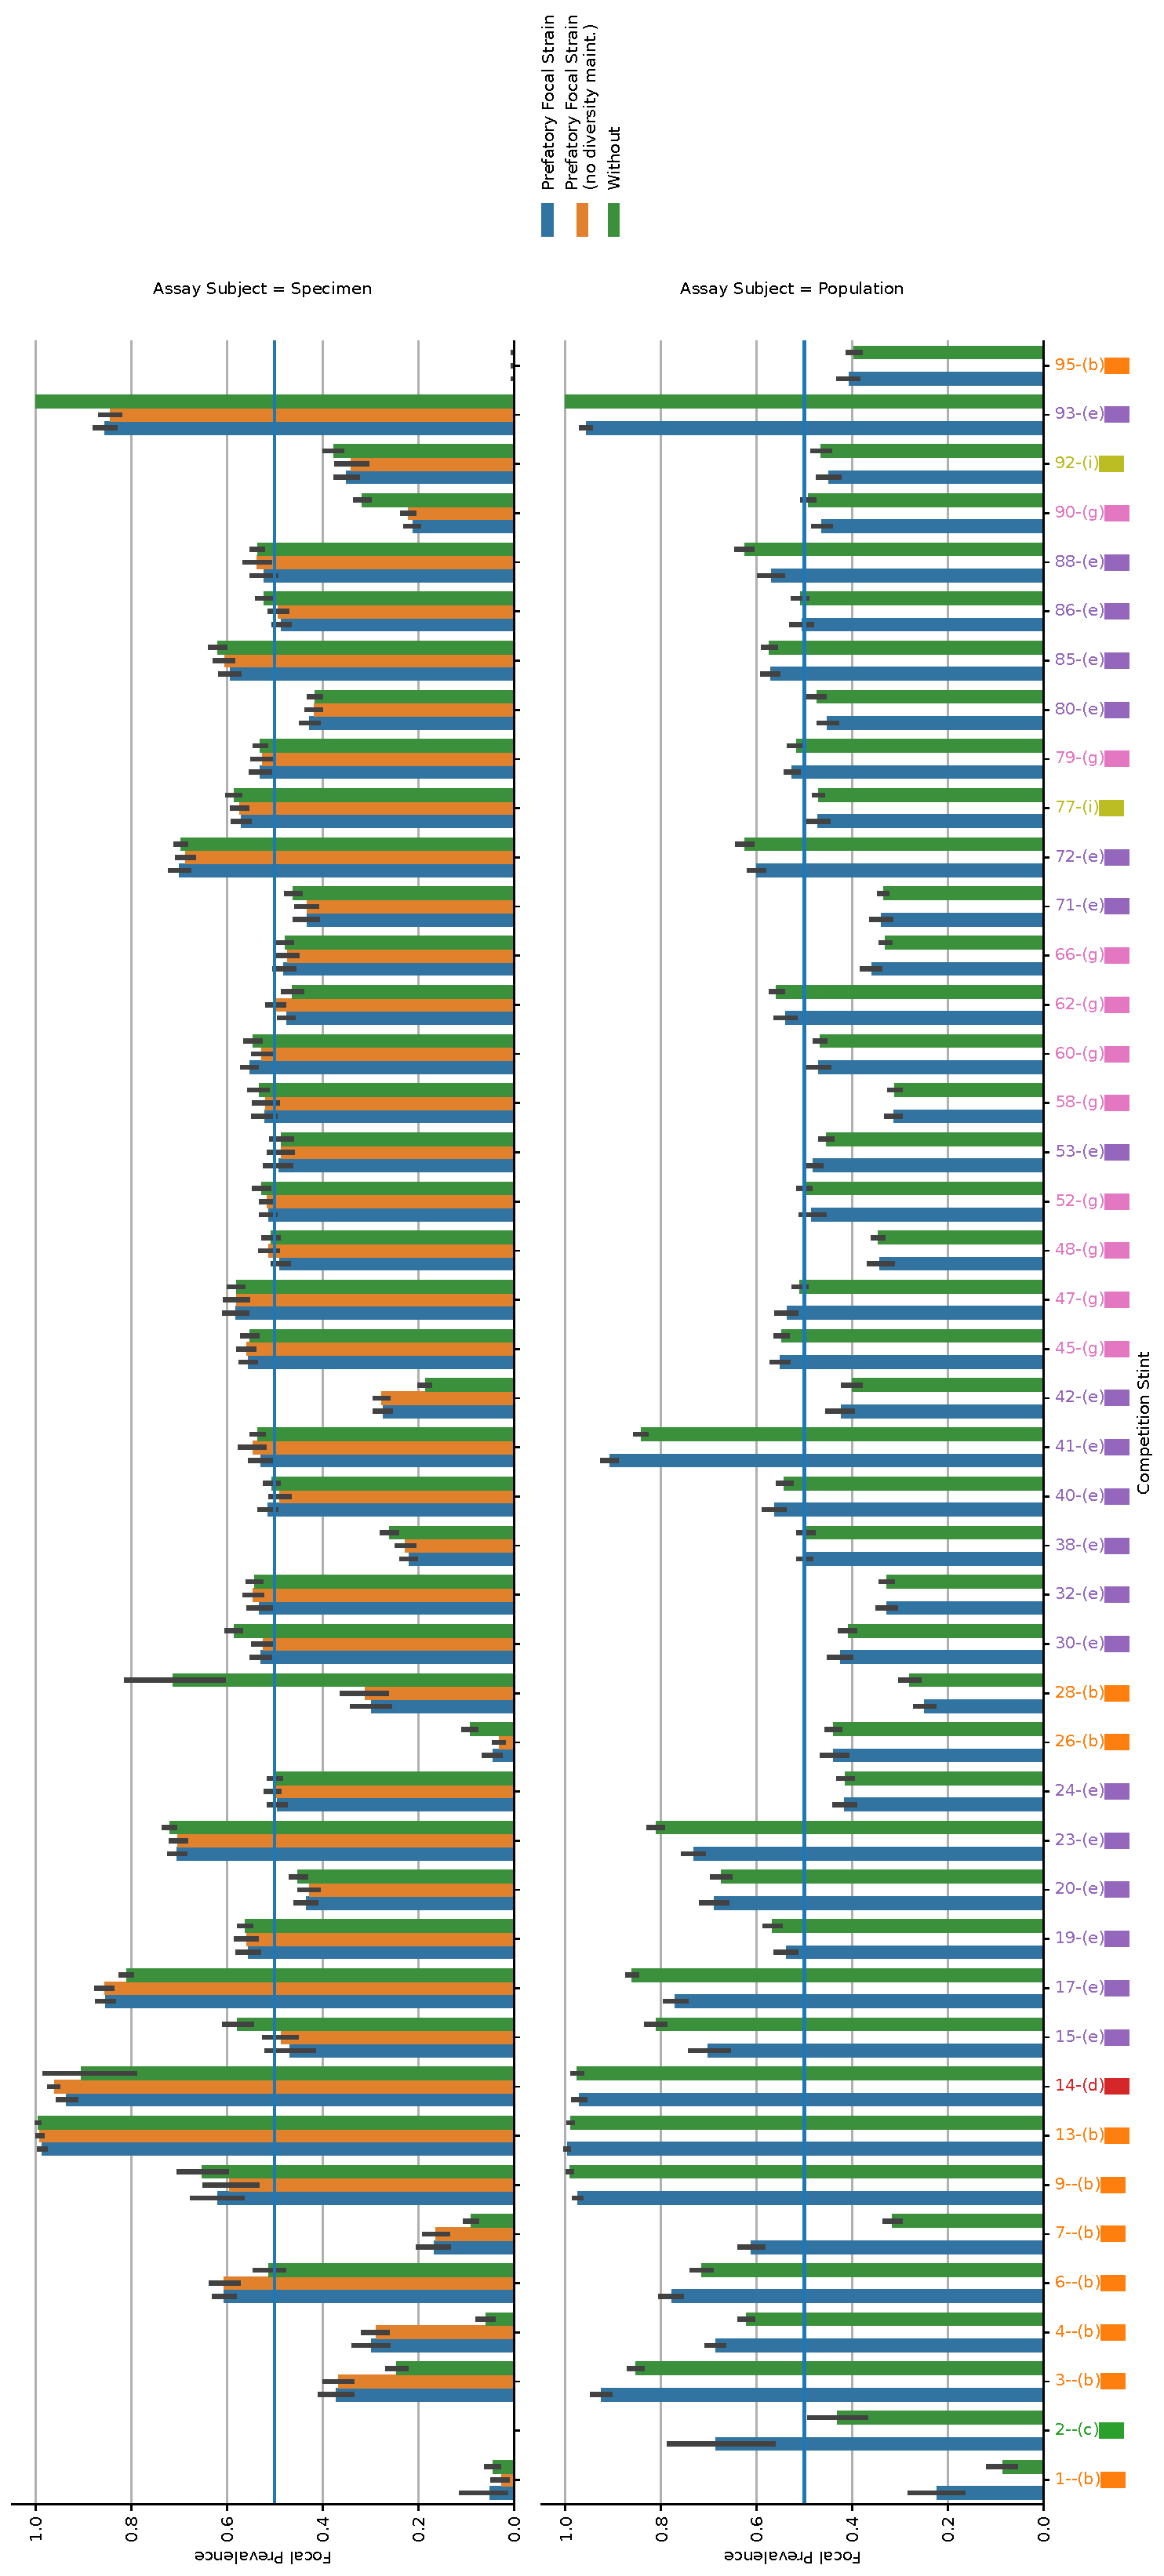
\includegraphics[width=0.7\linewidth]{{submodule/dishtiny/binder/bucket=prq49/a=adaptation_assays+endeavor=16/teeplots/a=baselinecontrol+hue=biotic-background+viz=facet-barplot+x=competition-stint+y=focal-prevalence+ext=}}
\caption{
Fractional composition of focal population at the end of competition experiments.
Zero is neutral.
Error bars are 95\% confidence intervals.
}
\end{subfigure}

\begin{subfigure}{\textwidth}
\centering
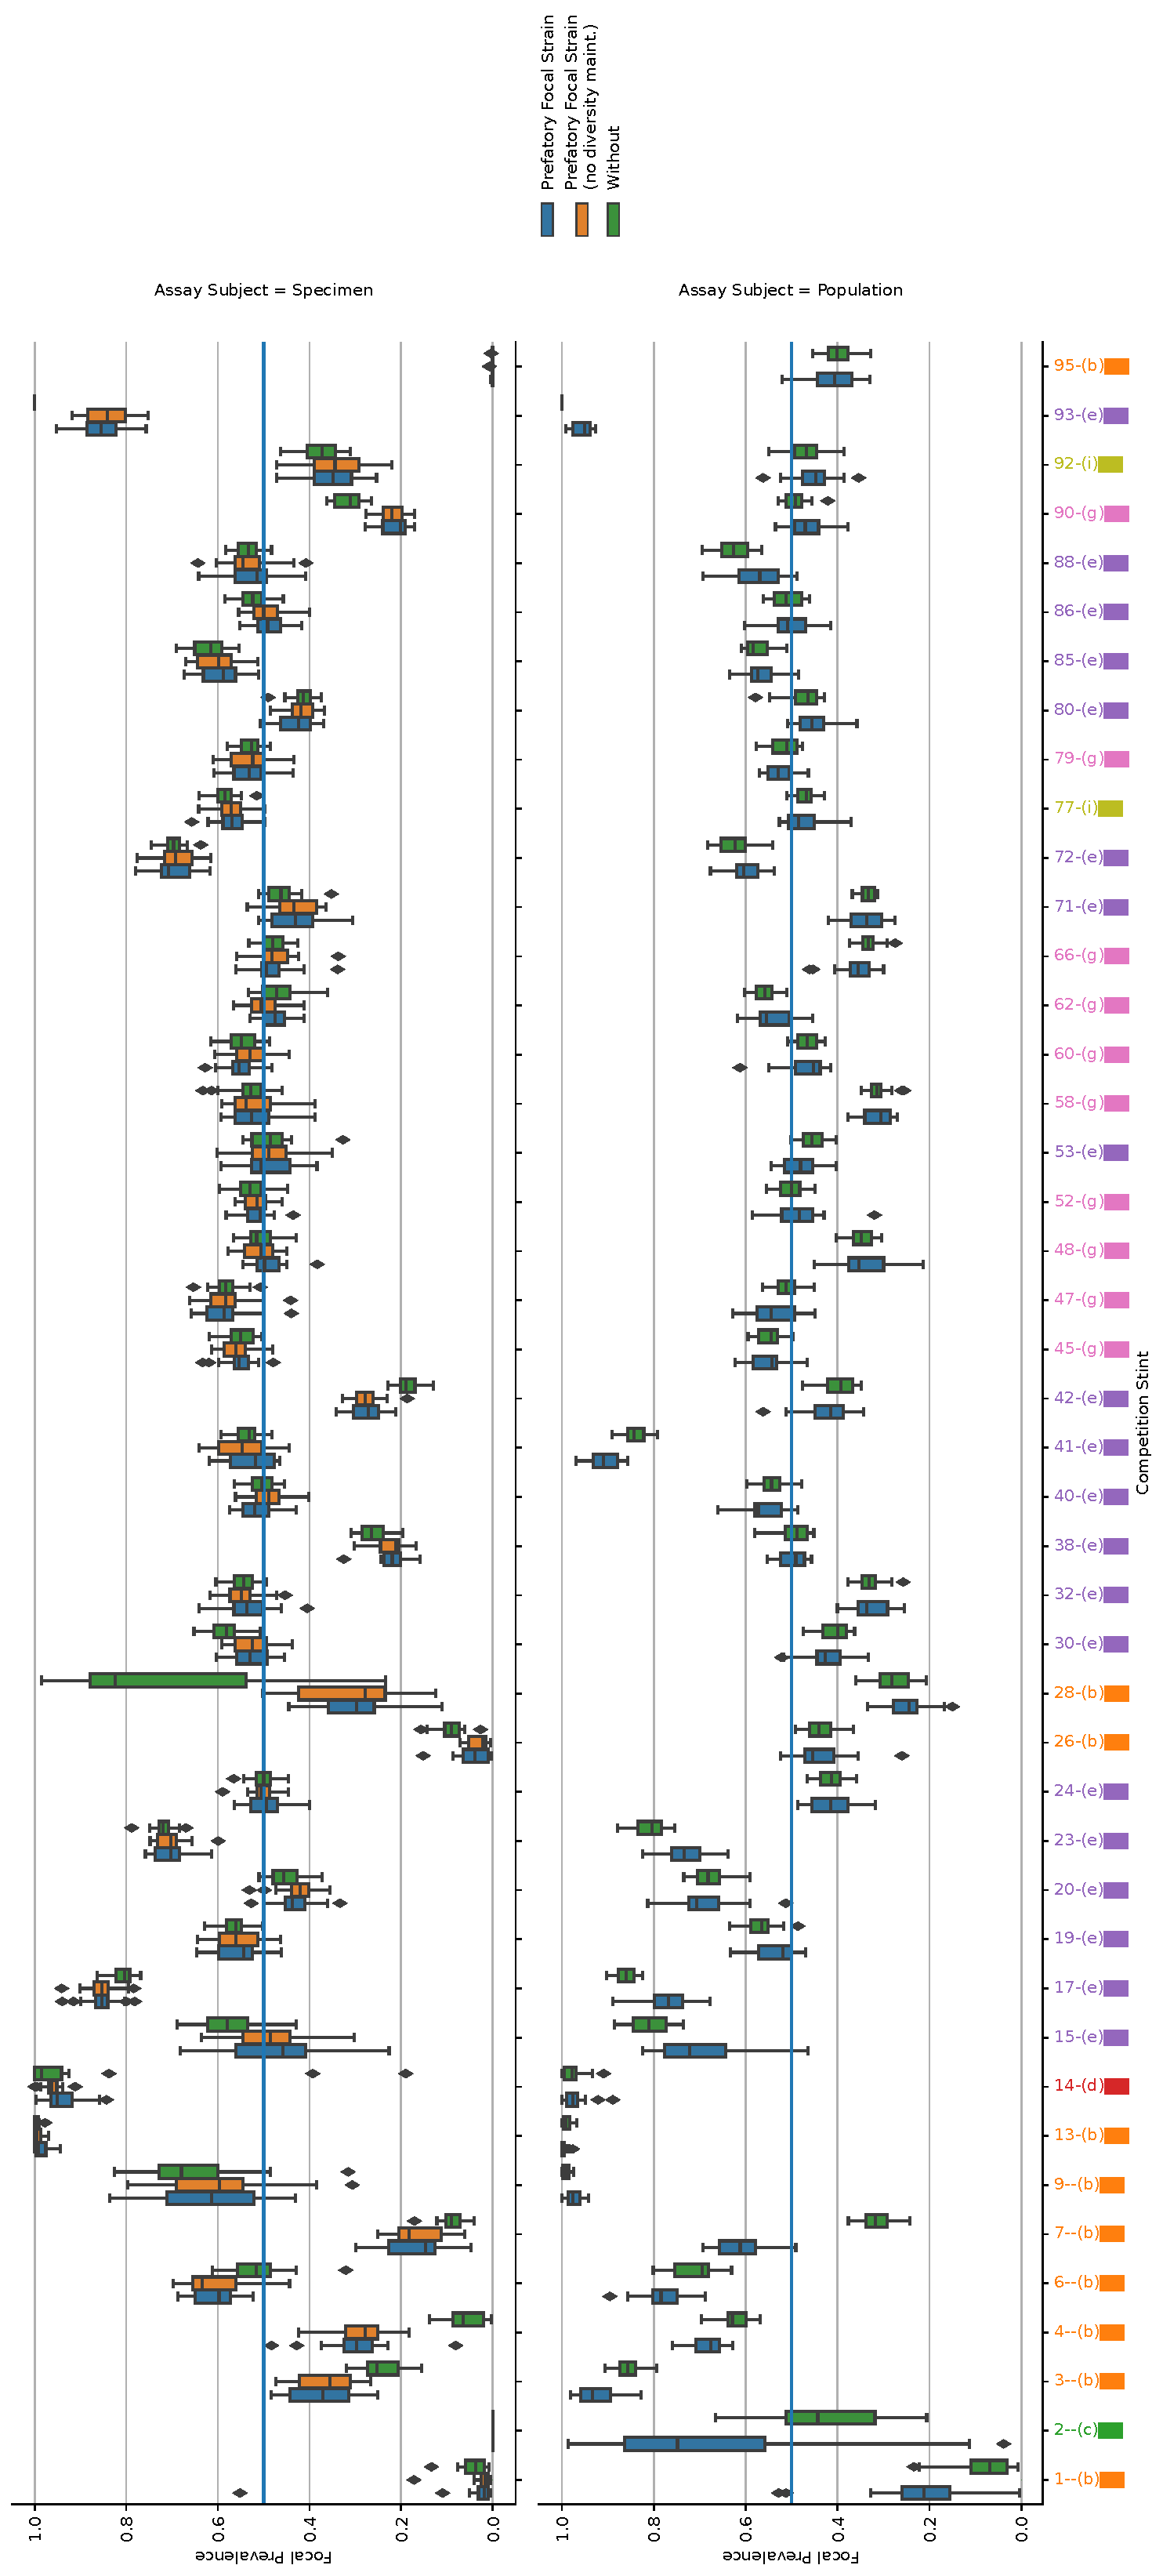
\includegraphics[width=0.7\linewidth]{{submodule/dishtiny/binder/bucket=prq49/a=adaptation_assays+endeavor=16/teeplots/a=baselinecontrol+hue=biotic-background+viz=facet-boxplot+x=competition-stint+y=focal-prevalence+ext=}}
\caption{
Fractional composition of focal population at the end of competition experiments.
A neutral outcome corresponds to even (0.5) composition, annotated with a horizontal line.
}
\end{subfigure}

\begin{subfigure}{\textwidth}
\centering
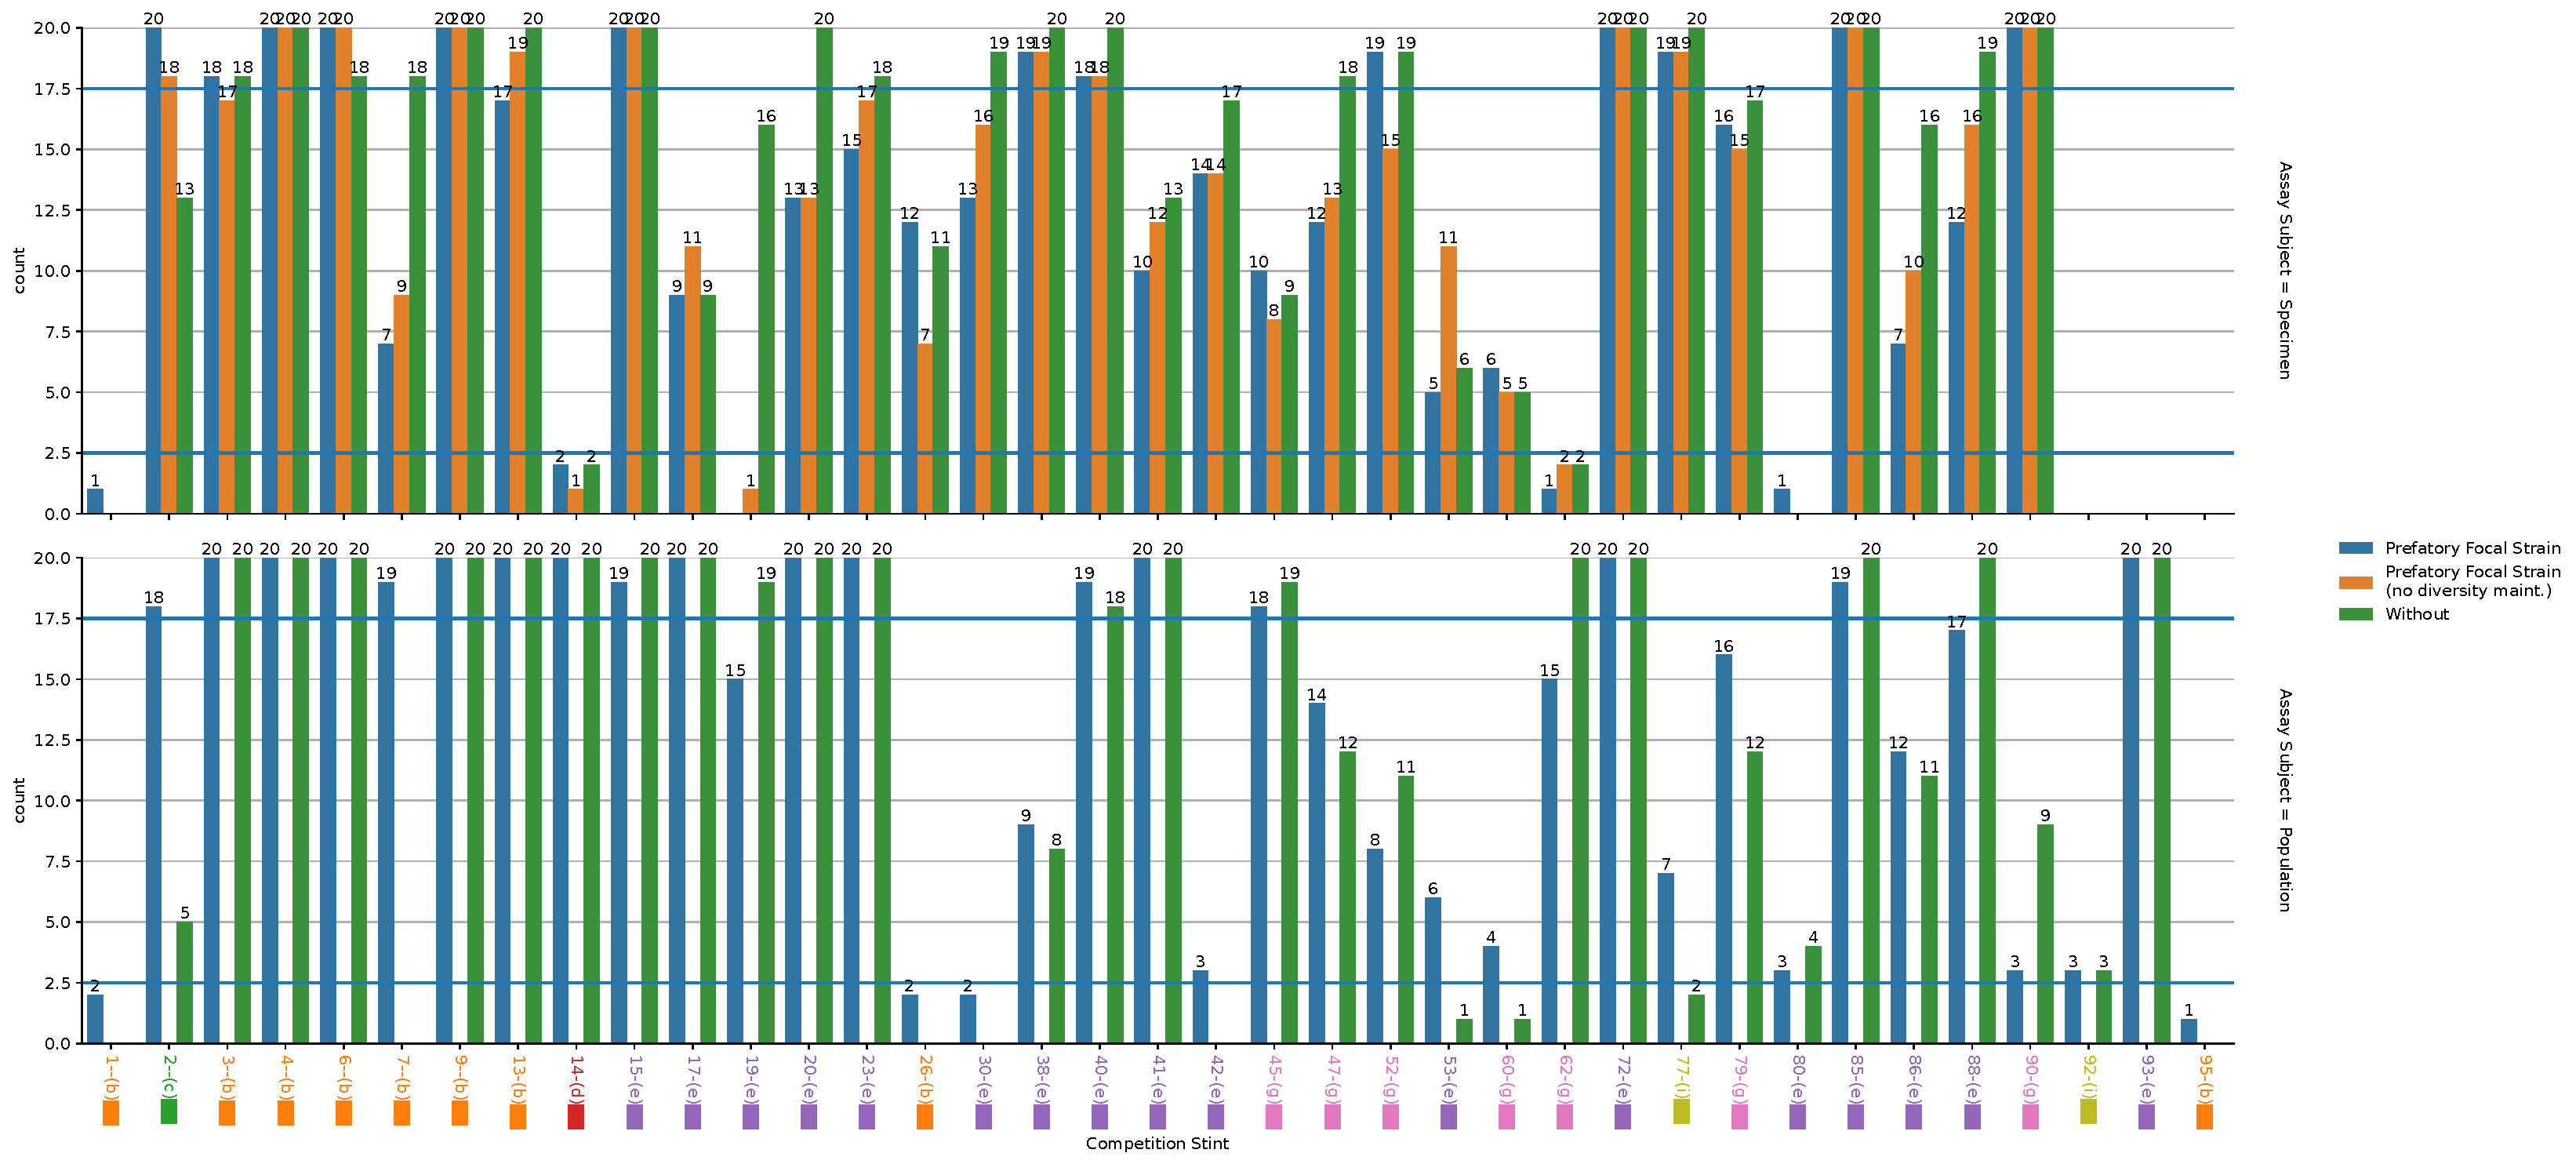
\includegraphics[width=0.7\linewidth]{{submodule/dishtiny/binder/bucket=prq49/a=adaptation_assays+endeavor=16/teeplots/a=baselinecontrol+hue=biotic-background+viz=facet-countplot+x=competition-stint+ext=}}
\caption{
Number competitions out of 20 won by first strain.
Ten competitions won corresponds to a perfectly neutral outcome.
Eighteen and more or two or less competitions won were considered to indicate a significant fitness difference between strains.
These thresholds for significance annotated with horizontal lines.
}
\end{subfigure}

\caption{
Biotic background control adaptation experiments for selected stints.
Biotic background control experiments were performed by substituting the baseline competitor for the biotic background.
See Figure \ref{fig:adaptation_assay_cartoon} for summary of adaptation experiment design.
}
\label{fig:baseline_adaptation_control}
\end{figure*}
